

\section{OpticalElement: \textquotedbl{}MICADO\_Sci\textquotedbl{}%
  \label{opticalelement-micado-sci}%
}

\textbf{Element}: instrument

\textbf{Alias}: INST

\textbf{Description}: base configuration for MICADO


\subsection{Global properties%
  \label{global-properties}%
}

\begin{quote}
\begin{alltt}
\begin{lstlisting}[frame=single]
       temperature : -190
filter_file_format : filters/TC_filter_\{\}.dat
      element_name : MICADO_Sci
\end{lstlisting}
\end{alltt}
\end{quote}


\subsection{Effects%
  \label{effects}%
}

Summary of Effects included in this optical element:

\setlength{\DUtablewidth}{\linewidth}
\begin{longtable*}[c]{|p{0.133\DUtablewidth}|p{0.249\DUtablewidth}|p{0.145\DUtablewidth}|p{0.110\DUtablewidth}|p{0.156\DUtablewidth}|}
\hline
\textbf{%
element
} & \textbf{%
name
} & \textbf{%
class
} & \textbf{%
included
} & \textbf{%
z\_orders {[}3{]}
} \\
\hline
\endfirsthead
\hline
\textbf{%
element
} & \textbf{%
name
} & \textbf{%
class
} & \textbf{%
included
} & \textbf{%
z\_orders {[}3{]}
} \\
\hline
\endhead
\multicolumn{5}{c}{\hfill ... continued on next page} \\
\endfoot
\endlastfoot

MICADO\_Sci
 & 
micado\_common\_optics
 & 
TERCurve
 & 
True
 & 
10 .. 510
 \\
\hline

MICADO\_Sci
 & 
filter\_wheel
 & 
FilterWheel
 & 
True
 & 
124 .. 524
 \\
\hline
\end{longtable*}
\label{tbl-micado-sci}


\subsubsection{TERCurve: \textquotedbl{}micado\_common\_optics\textquotedbl{}%
  \label{tercurve-micado-common-optics}%
}

\textbf{Included by default}: \texttt{True}

\textbf{File Description}: combined transmission for MICADO common optics

\textbf{Class Description}: Transmission, Emissivity, Reflection Curve

\textbf{Changes}:

\begin{itemize}
\item \end{itemize}


\paragraph{Data%
  \label{data}%
}

\begin{figure}[H]
\noindent\makebox[\linewidth][c]{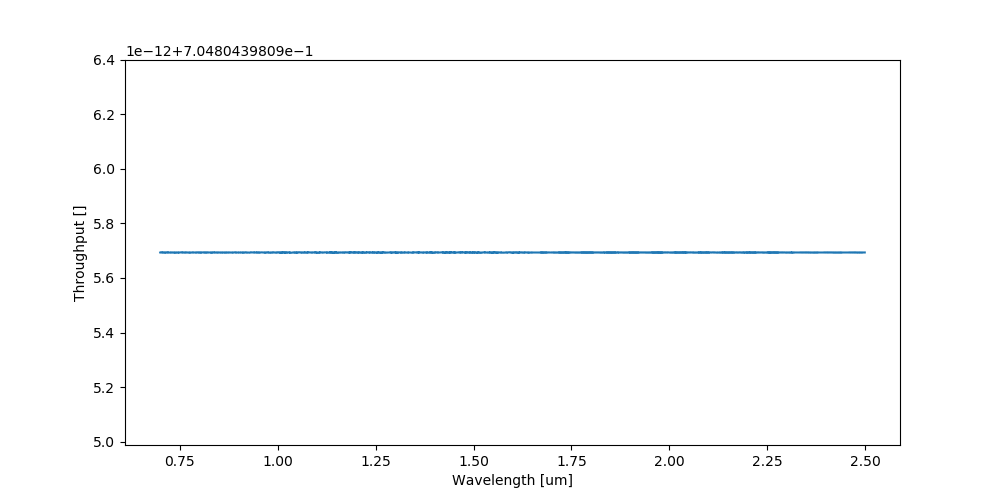
\includegraphics{micado_common_optics.png}}\phantomsection\label{fig-micado-common-optics}
\end{figure}


\paragraph{Meta-data%
  \label{meta-data}%
}

\begin{quote}
\begin{alltt}
\begin{lstlisting}[frame=single]
            filename : TER_MICADO_IMG_common.dat
                name : micado_common_optics
         temperature : -190
  filter_file_format : filters/TC_filter_\{\}.dat
        element_name : MICADO_Sci
              author : Auto-compiled from source
              source : LIST_MICADO_mirrors_static.dat
        date_created : 2020-08-25
       date_modified : 2020-08-25
                area : 0.19634954084936207
           area_unit : m2
     wavelength_unit : um
       emission_unit : photlam
             z_order : [10, 110, 510]
             include : True
        ignore_wings : False
            wave_min : 0.7
            wave_max : 2.5
           wave_unit : um
            wave_bin : 0.001
 report_plot_include : True
report_table_include : False
\end{lstlisting}
\end{alltt}
\end{quote}


\subsubsection{FilterWheel: \textquotedbl{}filter\_wheel\textquotedbl{}%
  \label{filterwheel-filter-wheel}%
}

\textbf{Included by default}: \texttt{True}

\textbf{File Description}:

\textbf{Class Description}: Examples

\textbf{Changes}:

\begin{itemize}
\item \end{itemize}


\paragraph{Data%
  \label{id1}%
}

\begin{figure}[H]
\noindent\makebox[\linewidth][c]{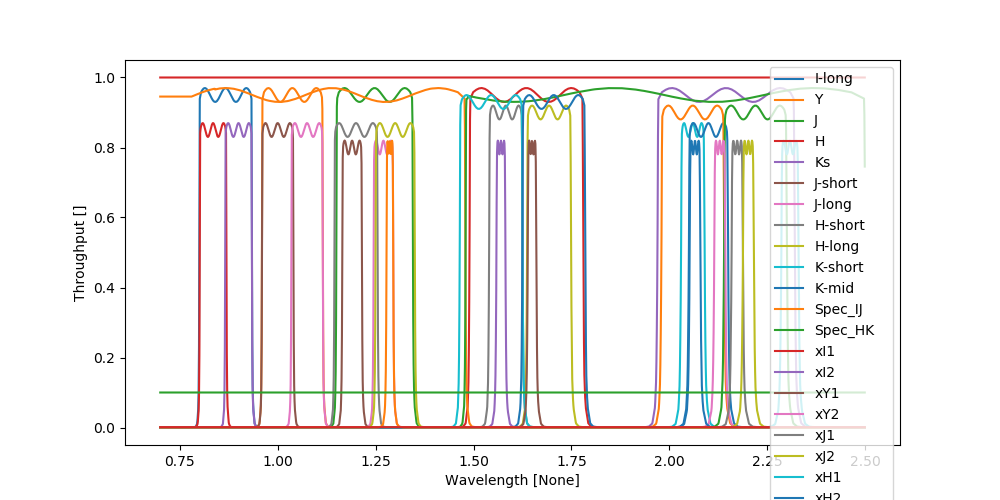
\includegraphics{filter_wheel.png}}\phantomsection\label{fig-filter-wheel}
\end{figure}

\setlength{\DUtablewidth}{\linewidth}
\begin{longtable*}[c]{|p{0.110\DUtablewidth}|p{0.086\DUtablewidth}|p{0.086\DUtablewidth}|p{0.145\DUtablewidth}|p{0.133\DUtablewidth}|}
\hline
\textbf{%
name
} & \textbf{%
\begin{description}
\item[{centre}] \leavevmode 
um

\end{description}
} & \textbf{%
\begin{description}
\item[{width}] \leavevmode 
um

\end{description}
} & \textbf{%
\begin{description}
\item[{blue cutoff}] \leavevmode 
um

\end{description}
} & \textbf{%
\begin{description}
\item[{red cutoff}] \leavevmode 
um

\end{description}
} \\
\hline
\endfirsthead
\hline
\textbf{%
name
} & \textbf{%
\begin{description}
\item[{centre}] \leavevmode 
um

\end{description}
} & \textbf{%
\begin{description}
\item[{width}] \leavevmode 
um

\end{description}
} & \textbf{%
\begin{description}
\item[{blue cutoff}] \leavevmode 
um

\end{description}
} & \textbf{%
\begin{description}
\item[{red cutoff}] \leavevmode 
um

\end{description}
} \\
\hline
\endhead
\multicolumn{5}{c}{\hfill ... continued on next page} \\
\endfoot
\endlastfoot

I-long
 & 
0.8689
 & 
0.1340
 & 
0.8019
 & 
0.9359
 \\
\hline

Y
 & 
1.0396
 & 
0.1550
 & 
0.9621
 & 
1.1171
 \\
\hline

J
 & 
1.2502
 & 
0.1950
 & 
1.1527
 & 
1.3477
 \\
\hline

H
 & 
1.6395
 & 
0.2900
 & 
1.4945
 & 
1.7845
 \\
\hline

Ks
 & 
2.1500
 & 
0.3500
 & 
1.9750
 & 
2.3250
 \\
\hline

J-short
 & 
1.1902
 & 
0.0490
 & 
1.1657
 & 
1.2147
 \\
\hline

J-long
 & 
1.2702
 & 
0.0490
 & 
1.2457
 & 
1.2947
 \\
\hline

H-short
 & 
1.5830
 & 
0.0850
 & 
1.5405
 & 
1.6255
 \\
\hline

H-long
 & 
1.6937
 & 
0.1120
 & 
1.6377
 & 
1.7497
 \\
\hline

K-short
 & 
2.0602
 & 
0.0600
 & 
2.0302
 & 
2.0902
 \\
\hline

K-mid
 & 
2.1005
 & 
0.1000
 & 
2.0505
 & 
2.1505
 \\
\hline

Spec\_IJ
 & 
1.1663
 & 
0.6990
 & 
0.8168
 & 
1.5158
 \\
\hline

Spec\_HK
 & 
2.0345
 & 
1.0200
 & 
1.5245
 & 
2.5445
 \\
\hline

xI1
 & 
0.8355
 & 
0.0680
 & 
0.8015
 & 
0.8695
 \\
\hline

xI2
 & 
0.9005
 & 
0.0680
 & 
0.8665
 & 
0.9345
 \\
\hline

xY1
 & 
1.0006
 & 
0.0800
 & 
0.9606
 & 
1.0406
 \\
\hline

xY2
 & 
1.0756
 & 
0.0800
 & 
1.0356
 & 
1.1156
 \\
\hline

xJ1
 & 
1.2009
 & 
0.1100
 & 
1.1459
 & 
1.2559
 \\
\hline

xJ2
 & 
1.3007
 & 
0.1000
 & 
1.2507
 & 
1.3507
 \\
\hline

xH1
 & 
1.5465
 & 
0.1600
 & 
1.4665
 & 
1.6265
 \\
\hline

xH2
 & 
1.7064
 & 
0.1600
 & 
1.6264
 & 
1.7864
 \\
\hline

xK1
 & 
2.0612
 & 
0.1600
 & 
1.9812
 & 
2.1412
 \\
\hline

xK2
 & 
2.2211
 & 
0.1600
 & 
2.1411
 & 
2.3011
 \\
\hline

blank
 & 
2.7545
 & 
2.7000
 & 
1.4045
 & 
4.1045
 \\
\hline

H-cont
 & 
1.5701
 & 
0.0220
 & 
1.5591
 & 
1.5811
 \\
\hline

FeII
 & 
1.6495
 & 
0.0210
 & 
1.6390
 & 
1.6600
 \\
\hline

H2\_1-0S1
 & 
2.1289
 & 
0.0280
 & 
2.1149
 & 
2.1429
 \\
\hline

Br-gamma
 & 
2.1734
 & 
0.0280
 & 
2.1594
 & 
2.1874
 \\
\hline

K-cont
 & 
2.2019
 & 
0.0270
 & 
2.1884
 & 
2.2154
 \\
\hline

K-long
 & 
2.3081
 & 
0.0440
 & 
2.2861
 & 
2.3301
 \\
\hline

He-I
 & 
2.0656
 & 
0.0270
 & 
2.0521
 & 
2.0791
 \\
\hline

Pa-beta
 & 
1.2865
 & 
0.0170
 & 
1.2780
 & 
1.2950
 \\
\hline

ND1
 & 
2.7529
 & 
0.0000
 & 
2.7529
 & 
2.7529
 \\
\hline

ND3
 & 
2.7529
 & 
0.0000
 & 
2.7529
 & 
2.7529
 \\
\hline
\end{longtable*}
\label{tbl-filter-wheel}


\paragraph{Meta-data%
  \label{id2}%
}

\begin{quote}
\begin{alltt}
\begin{lstlisting}[frame=single]
             filename : None
                 name : filter_wheel
          temperature : -190
   filter_file_format : filters/TC_filter_\{\}.dat
         element_name : MICADO_Sci
         filter_names : ['I-long', 'Y', 'J', 'H', 'Ks', 'J-short', 'J-long', 'H-short', 'H-long', 'K-short', 'K-mid', 'Spec_IJ', 'Spec_HK', 'xI1', 'xI2', 'xY1', 'xY2', 'xJ1', 'xJ2', 'xH1', 'xH2', 'xK1', 'xK2', 'blank', 'H-cont', 'FeII', 'H2_1-0S1', 'Br-gamma', 'K-cont', 'K-long', 'He-I', 'Pa-beta', 'ND1', 'ND3']
      filename_format : !INST.filter_file_format
       current_filter : !INST.filter_name
   minimum_throughput : 0.000101
                outer : 0.2
           outer_unit : m
              z_order : [124, 224, 524]
              include : True
                 path :
  report_plot_include : True
 report_table_include : True
report_table_rounding : 4
\end{lstlisting}
\end{alltt}
\end{quote}
